% Auto-generated by generate_report.py — do not edit manually
% Preamble mirrors oxengthesis.cls so figures match the body text:
% Carlito as main font, Latin Modern Math via unicode-math.
\documentclass[border=6pt]{standalone}
\usepackage{fontspec}
\setmainfont{Carlito}
\usepackage{unicode-math}
\setmathfont{Latin Modern Math}
\usepackage{pgfplots}
\pgfplotsset{compat=1.18}
\usepgfplotslibrary{groupplots}
\usetikzlibrary{patterns,positioning}
\begin{document}
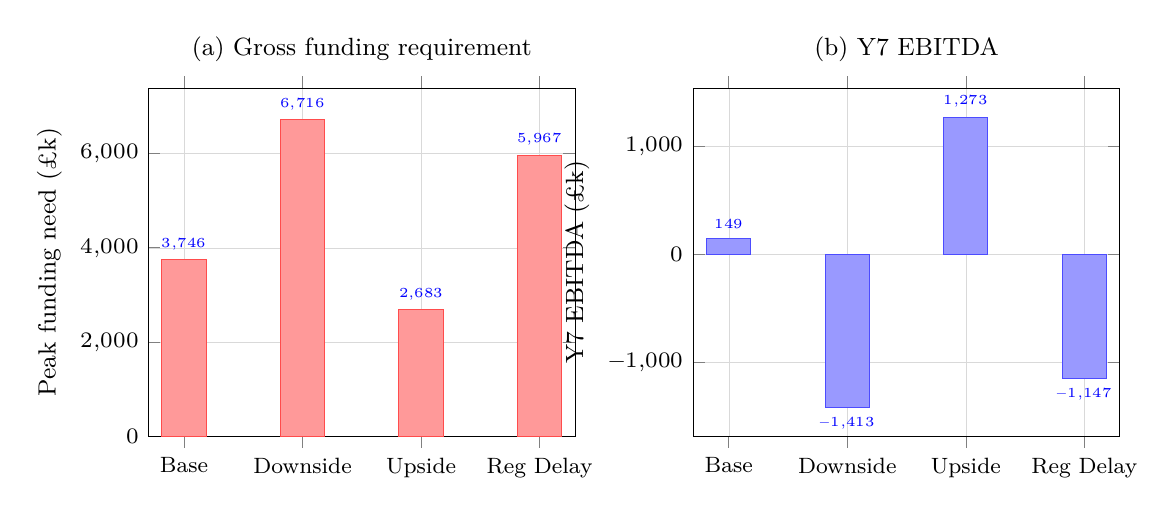
\begin{tikzpicture}
    \begin{axis}[
        width=7cm,
        height=6cm,
        name=left,
        ybar,
        bar width=16pt,
        ylabel={Peak funding need (\pounds k)},
        symbolic x coords={{Base},{Downside},{Upside},{Reg Delay}},
        xtick=data,
        ymin=0,
        nodes near coords,
        nodes near coords style={font=\tiny},
        grid=major,
        grid style={line width=.1pt, draw=gray!30},
        tick label style={font=\footnotesize},
        label style={font=\small},
        title={(a) Gross funding requirement},
        title style={font=\small},
    ]
    \addplot+[ybar,fill=red!40,draw=red!70] coordinates {({Base},3746) ({Downside},6716) ({Upside},2683) ({Reg Delay},5967)};
    \end{axis}
    \begin{axis}[
        width=7cm,
        height=6cm,
        at=(left.east), anchor=west, xshift=1.5cm,
        ybar,
        bar width=16pt,
        ylabel={Y7 EBITDA (\pounds k)},
        symbolic x coords={{Base},{Downside},{Upside},{Reg Delay}},
        xtick=data,
        nodes near coords,
        nodes near coords style={font=\tiny},
        grid=major,
        grid style={line width=.1pt, draw=gray!30},
        tick label style={font=\footnotesize},
        label style={font=\small},
        title={(b) Y7 EBITDA},
        title style={font=\small},
    ]
    \addplot+[ybar,fill=blue!40,draw=blue!70] coordinates {({Base},149) ({Downside},-1413) ({Upside},1273) ({Reg Delay},-1147)};
    \end{axis}
\end{tikzpicture}

\end{document}
